\documentclass{beamer}

\usepackage[utf8]{inputenc}
\usepackage{hyperref}

\usetheme{Berkeley}
\beamertemplatenavigationsymbolsempty
\setbeamertemplate{headline}{}
 
\title{Geocoding with Photon in FoodChain-Lab}
%\subtitle{Geocoding with Photon}
\date{}
 
\begin{document}
\maketitle

\section{ }

\subsection{Tasks}
\begin{frame}
	\begin{itemize}
		\item Perform a geocoding by using the Geocoding workflow from \url{https://github.com/SiLeBAT/BfROpenLabResources/raw/master/GitHubPages/workflows/Geocoding_with_Photon.knwf}.
		\item Add the \textbf{FoodChain-Lab} \textbf{Geocoding} node.
		\item Do the geocoding by using the Photon Geocoding Service.
	\end{itemize}
\end{frame}
 
\subsection{1}
\begin{frame}
	\begin{center}
  		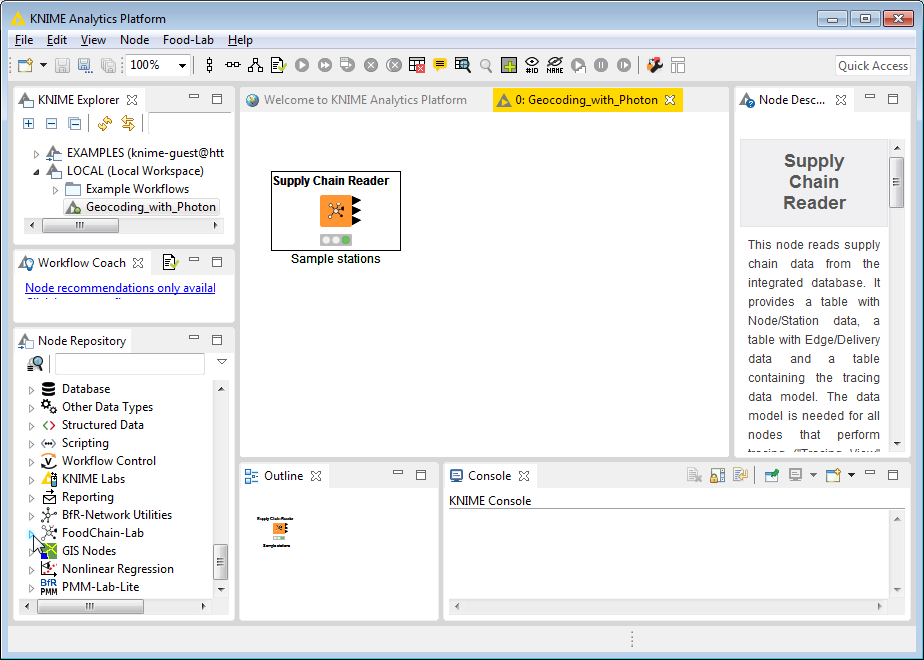
\includegraphics[height=0.6\textheight]{1.png}
	\end{center}
	\begin{itemize}
		\item Import the Geocoding workflow from \url{https://github.com/SiLeBAT/BfROpenLabResources/raw/master/GitHubPages/workflows/Geocoding_with_Photon.knwf}.
		%\item In this tutorial we are using the Photon Geocoding service.
	\end{itemize}
\end{frame}

\subsection{2}
\begin{frame}
	\begin{center}
  		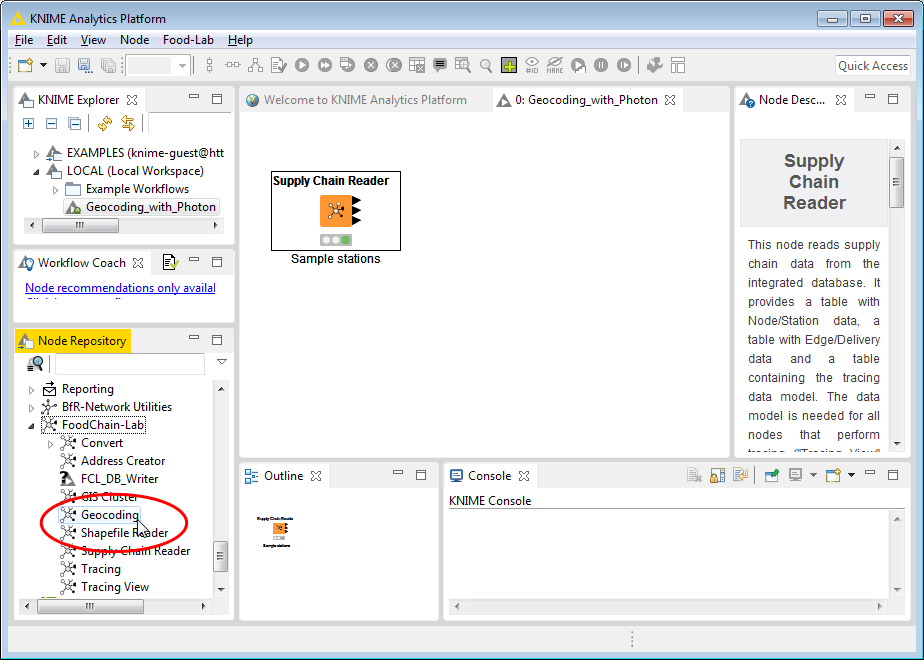
\includegraphics[height=0.6\textheight]{2.png}
	\end{center}
	\begin{itemize}
        \item To perform geocoding we need to add the \textbf{FoodChain-Lab} \textbf{Geocoding} node.
		\item Add the \textbf{FoodChain-Lab} \textbf{Geocoding} node by double clicking on it in the \textbf{Node Repository}.
		%\item In this tutorial we are using the Photon Geocoding service.
	\end{itemize}
\end{frame}

\subsection{3}
\begin{frame}
	\begin{center}
  		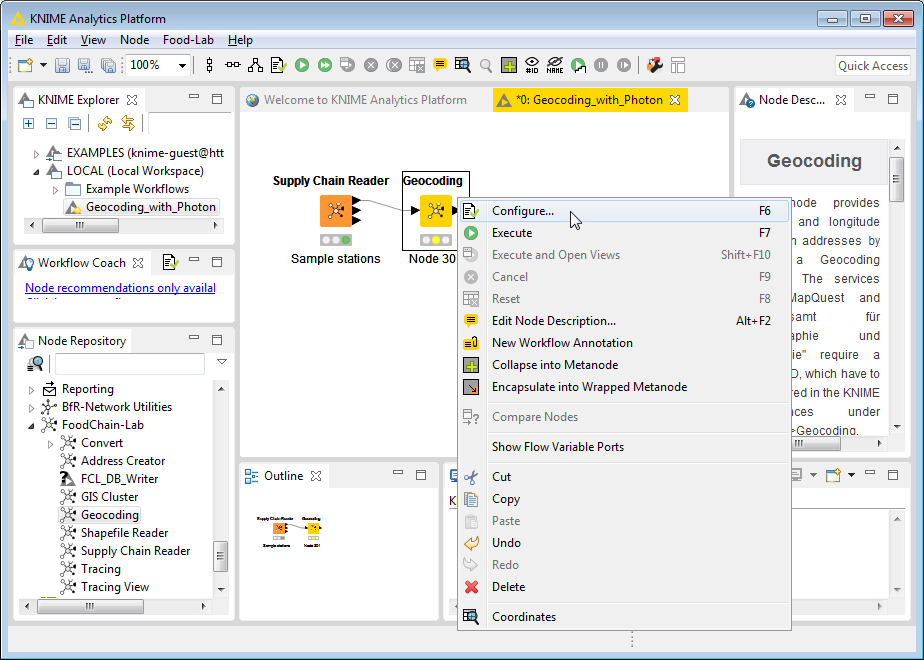
\includegraphics[height=0.6\textheight]{3.png}
	\end{center}
	\begin{itemize}
        \item A \textbf{Geocoding} node was added to the workflow. It is connected to the \textbf{SupplyChainReader} and needs to be set up.
		%\item The \textbf{Geocoding} node has to be set up (to use Photon)
		\item Open its configuration by double clicking on it or by using its context menue (right click on the node).
		%\item In this tutorial we are using the Photon Geocoding service.
	\end{itemize}
\end{frame}

\subsection{4}
\begin{frame}
	\begin{center}
  		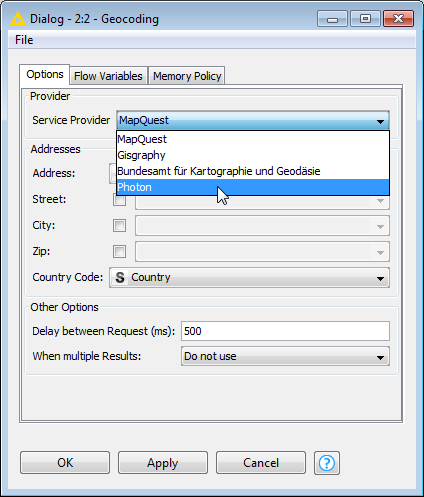
\includegraphics[height=0.6\textheight]{4.png}
	\end{center}
	\begin{itemize}
        \item Set the \textbf{Service Provider} to \textbf{Photon}.
		%\item The Geocoding-Node has to be configured (to use Photon)
		%\item Open its configuration by double clicking on it or by using its context menue (right click on the node)
		%\item In this tutorial we are using the Photon Geocoding service.
	\end{itemize}
\end{frame}

\subsection{5}
\begin{frame}
	\begin{center}
  		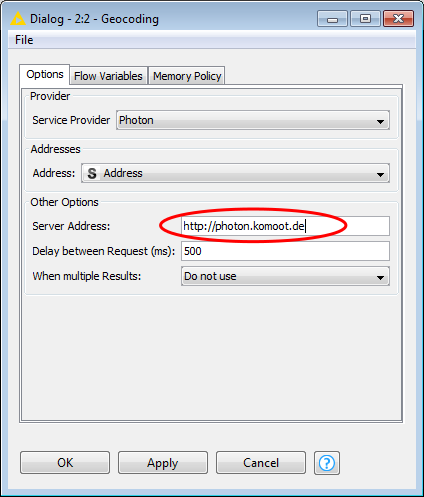
\includegraphics[height=0.6\textheight]{5.png}
	\end{center}
	\begin{itemize}
        \item The \textbf{Address} is properly set
		\item You need to set the \textbf{Server Address}. You can use \textbf{http://photon.komoot.de}, which is a public available service. 
		%\item The Geocoding-Node has to be configured (to use Photon)
		%\item Open its configuration by double clicking on it or by using its context menue (right click on the node)
		%\item In this tutorial we are using the Photon Geocoding service.
	\end{itemize}
\end{frame}

\subsection{6}
\begin{frame}
	\begin{center}
  		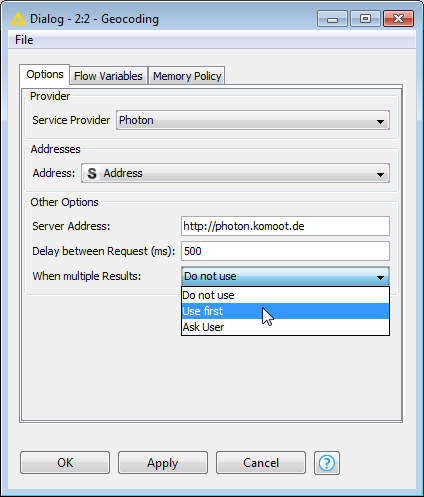
\includegraphics[height=0.5\textheight]{6.png}
	\end{center}
	\begin{itemize}
		\item For many requests geocoding services return multiple results (e.g. when there are two streets with the same name).
		\item To deal with this we have to decide if we just want to use the first or look at all choices and try to find the best.
		\item Looking manually at all choices is a lot of work for large data sets. In this tutorial select \textbf{Use first} and press \textbf{OK}.
	\end{itemize}
\end{frame}

\subsection{7}
\begin{frame}
	\begin{center}
  		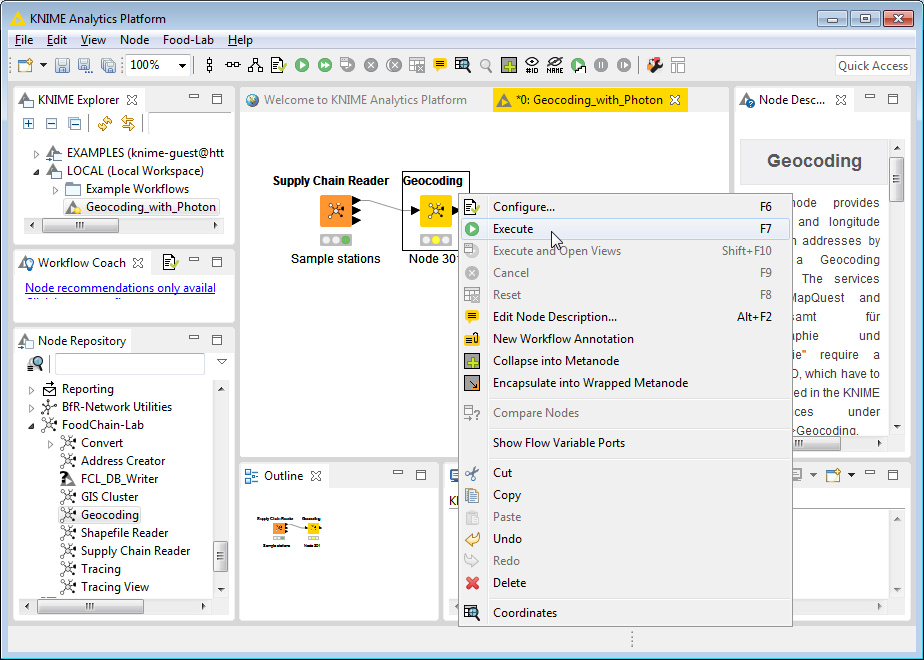
\includegraphics[height=0.6\textheight]{7.png}
	\end{center}
	\begin{itemize}
		\item Right click on the \textbf{Geocoding} node and select \textbf{Execute}.
	\end{itemize}
\end{frame}

\subsection{8}
\begin{frame}
	\begin{center}
  		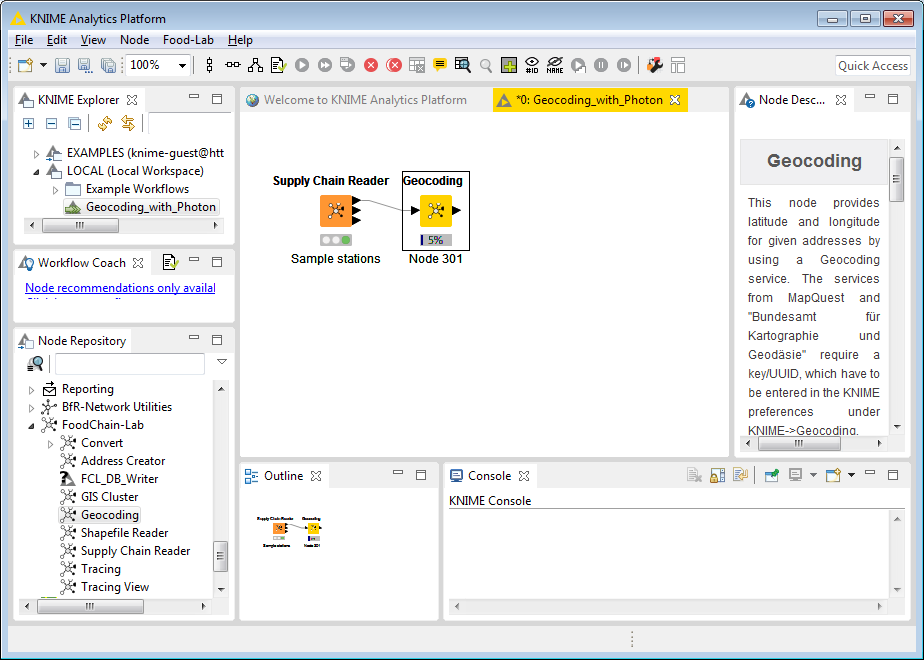
\includegraphics[height=0.6\textheight]{8.png}
	\end{center}
	\begin{itemize}
		\item The execution can take a while.
		\item The progress bar under the node shows what percentage of data has been processed.
	\end{itemize}
\end{frame}

\subsection{9}
\begin{frame}
	\begin{center}
  		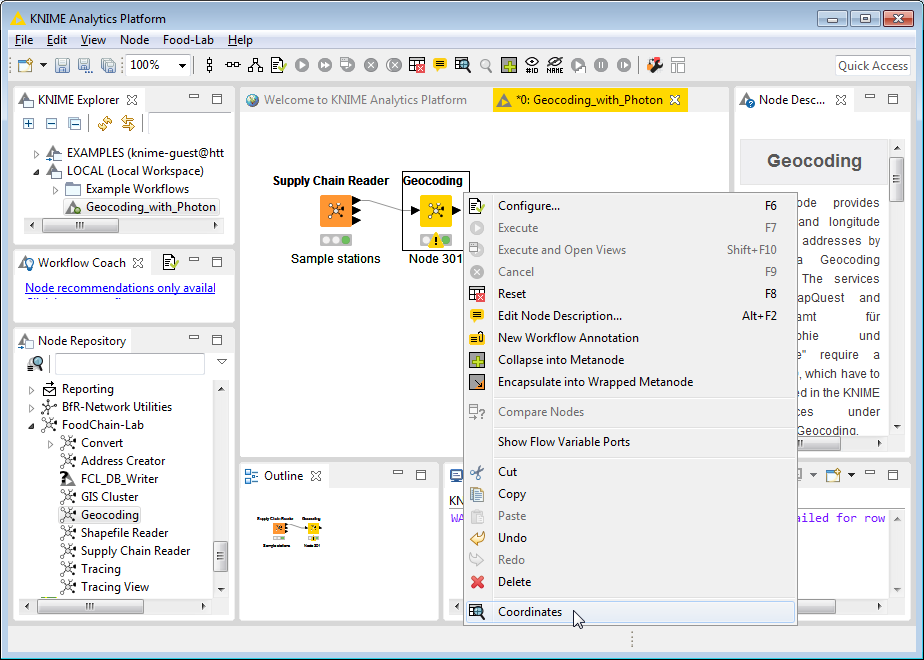
\includegraphics[height=0.6\textheight]{9.png}
	\end{center}
	\begin{itemize}
		\item When the execution is finished, we can look at the results.
		\item Right click on the \textbf{Geocoding} node and select \textbf{Coordinates}.
	\end{itemize}
\end{frame}

\subsection{10}
\begin{frame}
	\begin{center}
  		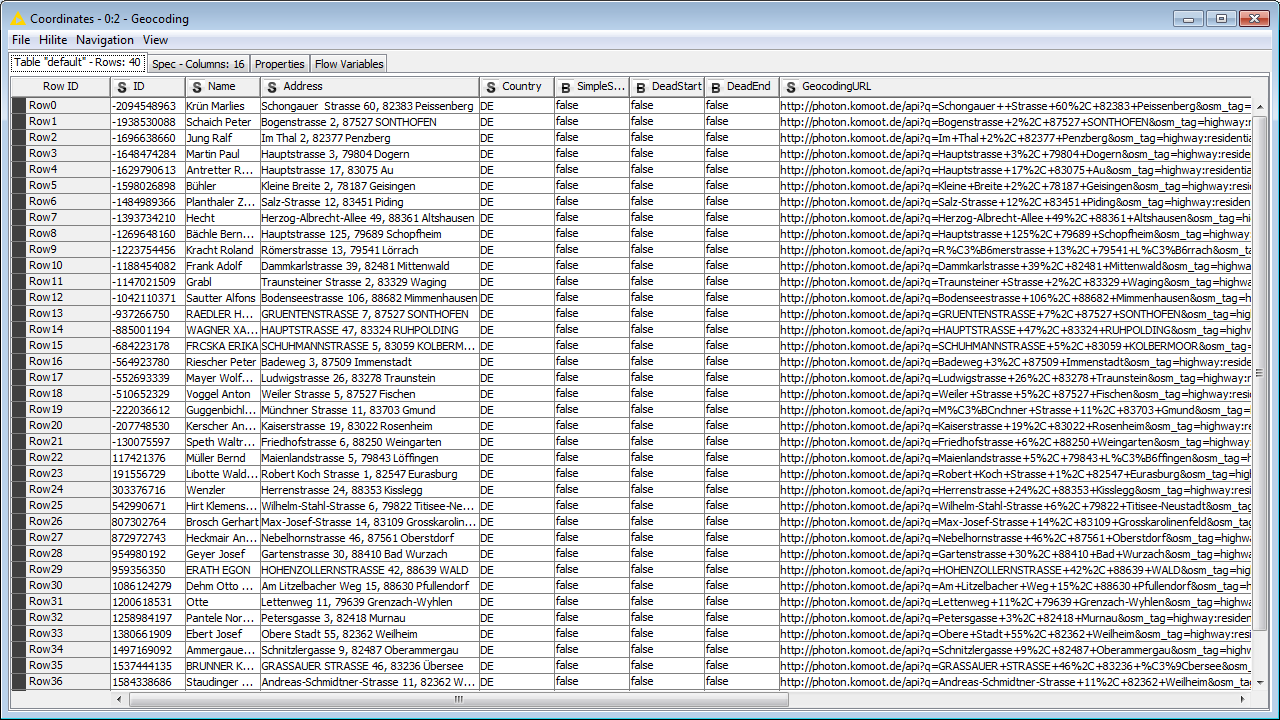
\includegraphics[height=0.6\textheight]{10.png}
	\end{center}
	\begin{itemize}
		\item In the dialog that pops up, you can look at the whole data table.
	\end{itemize}
\end{frame}

\subsection{11}
\begin{frame}
	\begin{center}
  		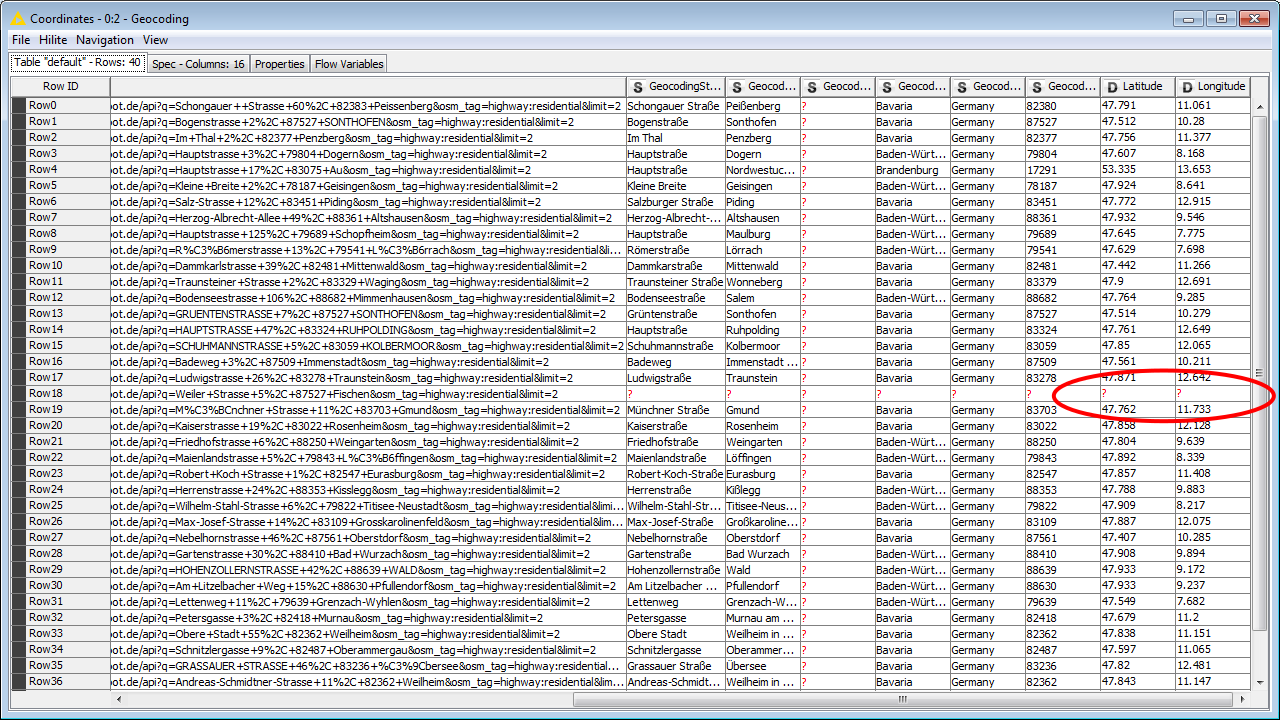
\includegraphics[height=0.6\textheight]{11.png}
	\end{center}
	\begin{itemize}
		\item Scroll to the right to look at the columns with latitude and longitude (the two rightmost columns).
		\item One geocoding request was not successful. 
	\end{itemize}
\end{frame}

\end{document}
